\documentclass[aspectratio=169, table, 12pt]{beamer}

% Preamble bersama seluruh slide mata kuliah ini.
% Dipanggil dari slides/sessionXX/sessionXX.tex tepat sesudah baris
% \documentclass[aspectratio=169, table, 12pt]{beamer}
% Paket tambahan yang hanya dibutuhkan satu sesi ditulis di berkas sesi itu.

\usepackage{colortbl}
\usepackage{xcolor}
\usepackage{listings}
\usepackage{tabularx}
\usepackage{booktabs}
\usepackage{tikz}
\usepackage{pgfplots}
\pgfplotsset{compat=1.18}
\usetikzlibrary{arrows.meta, positioning, calc, fit, shapes.geometric,
	shapes.multipart, backgrounds, matrix, chains, trees}

\makeatletter
\def\input@path{{../theme/}}
\makeatother
\graphicspath{{../theme/}{../../figures/}}
\usetheme{Pradita}

\definecolor{praditagreen}{RGB}{37, 113, 71}

% Tema membuat garis tabel berwarna putih. Dikembalikan agar tabel terbaca.
\arrayrulecolor{black}
\setlength{\arrayrulewidth}{0.5pt}

\lstdefinelanguage{yaml}{
	basicstyle=\ttfamily\scriptsize,
	keywordstyle=\color{blue}\bfseries,
	commentstyle=\color{gray}\itshape,
	stringstyle=\color{red},
	showstringspaces=false,
	breaklines=true,
	frame=lines,
	numbers=none,
	backgroundcolor=\color{lightgray!10},
	tabsize=2,
	morecomment=[l]{\#}
}

\lstdefinelanguage{json}{
	basicstyle=\ttfamily\scriptsize,
	stringstyle=\color{red},
	commentstyle=\color{gray},
	breaklines=true,
	showstringspaces=false,
	tabsize=2,
	numbers=none,
	frame=lines,
	backgroundcolor=\color{lightgray!10},
	string=[s]{"}{"}
}

\lstdefinelanguage{bash}{
	keywords={},
	basicstyle=\ttfamily\scriptsize,
	ndkeywords={docker, kubectl, helm, curl, git, terraform},
	ndkeywordstyle=\color{purple}\bfseries,
	sensitive=true,
	commentstyle=\color{gray},
	numbers=none,
	breaklines=true,
	frame=lines,
	backgroundcolor=\color{lightgray!10},
	tabsize=2,
	comment=[l]{\#},
	showstringspaces=false
}

\lstdefinelanguage{http}{
	keywords={GET, POST, PUT, PATCH, DELETE, HEAD, OPTIONS, HTTP},
	basicstyle=\ttfamily\scriptsize,
	keywordstyle=\color{blue}\bfseries,
	sensitive=true,
	numbers=none,
	breaklines=true,
	frame=lines,
	backgroundcolor=\color{lightgray!10},
	tabsize=2,
	showstringspaces=false
}

\subtitle{IT40713 · Cloud-Native \& Microservices Architecture}
\author{\textbf{Alfa Yohannis}}


\title{\Huge Orientasi dan Bahasa\\ \vspace{10pt} Bersama Cloud-Native}

\begin{document}

\frame{\titlepage}

\begin{frame}
  \frametitle{Isi Pertemuan}
  \vspace{10pt}
  \begin{columns}[t]
    \column{0.5\textwidth}
    {\small\tableofcontents[sections={1-4}]}

    \column{0.5\textwidth}
    {\small\tableofcontents[sections={5-8}]}
  \end{columns}
\end{frame}

\begin{frame}{\hfill}
  \centering
  \LARGE{\textbf{Kalau semua sistem dipindahkan\\ke \textit{cloud}, apakah
  masalahnya\\selesai?}}
\end{frame}

\section{Tujuan dan Kerangka Bahasan}

\begin{frame}{\hfill}
  \centering
  \Huge{\textbf{Tujuan dan Kerangka Bahasan}}
\end{frame}

\begin{frame}{Tujuan Pembelajaran}
  \vspace{6pt}
  \begin{itemize}
    \item Menjelaskan dengan bahasa sehari-hari istilah dasar sistem informasi:
          aplikasi, server, basis data, jaringan, pusat data, dan \textit{cloud}.
    \item Mengaitkan keputusan teknologi dengan nilai bisnis, biaya, risiko, dan
          regulasi.
    \item Merumuskan masalah teknologi informasi di organisasi pilihan tim sebagai
          pemicu modernisasi.
  \end{itemize}
\end{frame}

\begin{frame}{Pertanyaan Direksi Medikara Health}
  \begin{itemize}
    \item Antrean pendaftaran Senin pagi masih panjang.
    \item Lima rumah sakit memakai SIMRS dengan versi berbeda: setiap mitra baru
          butuh lima sambungan.
    \item Biaya integrasi terus naik.
    \item Jawaban "pindah ke \textit{cloud}" tidak otomatis menyelesaikan ketiganya:
          penyebabnya bisa di proses, rancangan aplikasi, atau server.
    \item Mata kuliah ini melatih cara menimbang pilihan beserta
          \textit{trade-off}-nya, lalu menuliskan justifikasinya.
  \end{itemize}
\end{frame}

\section{Cara Kerja Mata Kuliah dan Capstone}

\begin{frame}{\hfill}
  \centering
  \Huge{\textbf{Cara Kerja Mata Kuliah\\dan Proyek Capstone}}
\end{frame}

\begin{frame}{Belajar Mandiri, Tatap Muka Sabtu}
  \begin{itemize}
    \item Modul dan slide dipelajari mandiri sebelum Sabtu.
    \item Sabtu dipakai untuk meninjau progres proyek capstone, bukan mengulang
          isi modul.
    \item Analogi: bimbingan tugas akhir. Pertemuan membahas draf yang sudah ada.
    \item Ritme pekan: baca bab, kerjakan Aktivitas bersama tim, bawa draf ke kelas.
    \item Dengan 8 tim dan 150 menit tatap muka, setiap tim mendapat sekitar 15
          menit.
  \end{itemize}
\end{frame}

\begin{frame}{Empat Mata Kuliah, Satu Cetak Biru}
  \centering
  \resizebox{!}{0.66\textheight}{% Empat mata kuliah peminatan menyumbang ke satu cetak biru, disusun lewat
% empat tonggak capstone. Dipakai di Bab 01 dan slide Pertemuan 01.
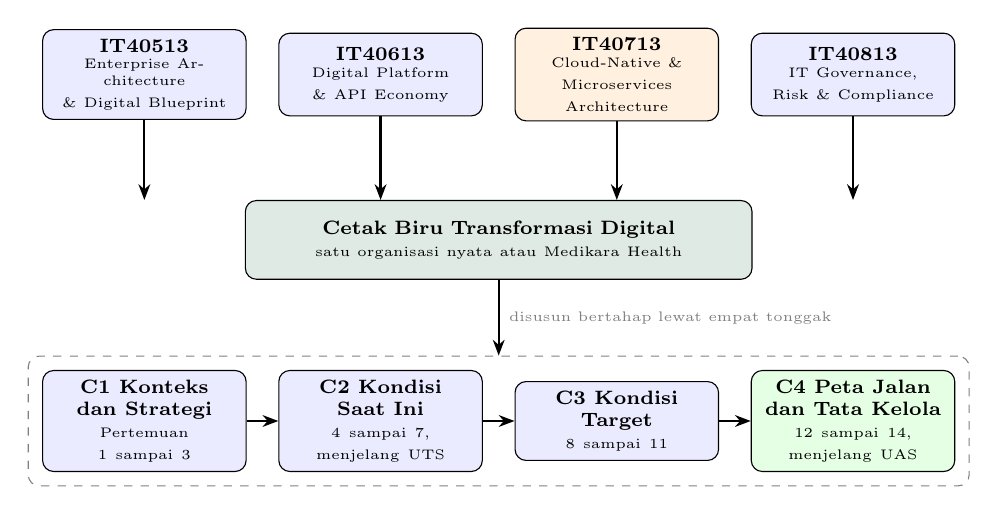
\begin{tikzpicture}[
  font=\scriptsize,
  kotak/.style={draw, rounded corners, align=center, minimum height=1.05cm,
                text width=2.35cm},
  tonggak/.style={draw, rounded corners, align=center, minimum height=0.95cm,
                  text width=2.35cm, font=\scriptsize\bfseries},
  panah/.style={-{Stealth[length=2mm]}, thick}
]
  \node[kotak, fill=blue!8] (ea) at (0,0)
    {\textbf{IT40513}\\{\tiny\mdseries Enterprise Architecture\\\& Digital Blueprint}};
  \node[kotak, fill=blue!8] (api) at (3,0)
    {\textbf{IT40613}\\{\tiny\mdseries Digital Platform\\\& API Economy}};
  \node[kotak, fill=orange!12] (cloud) at (6,0)
    {\textbf{IT40713}\\{\tiny\mdseries Cloud-Native \&\\Microservices Architecture}};
  \node[kotak, fill=blue!8] (grc) at (9,0)
    {\textbf{IT40813}\\{\tiny\mdseries IT Governance,\\Risk \& Compliance}};

  \node[draw, rounded corners, align=center, fill=praditagreen!15,
        text width=6.2cm, minimum height=1cm] (cetak) at (4.5,-2.1)
    {\textbf{Cetak Biru Transformasi Digital}\\
     {\tiny\mdseries satu organisasi nyata atau Medikara Health}};

  \foreach \asal in {ea, api, cloud, grc} {
    \draw[panah] (\asal.south) -- (\asal.south |- cetak.north);
  }

  \node[tonggak, fill=blue!8] (c1) at (0,-4.4)
    {C1 Konteks\\dan Strategi\\{\tiny\mdseries Pertemuan 1 sampai 3}};
  \node[tonggak, fill=blue!8] (c2) at (3,-4.4)
    {C2 Kondisi\\Saat Ini\\{\tiny\mdseries 4 sampai 7, menjelang UTS}};
  \node[tonggak, fill=blue!8] (c3) at (6,-4.4)
    {C3 Kondisi\\Target\\{\tiny\mdseries 8 sampai 11}};
  \node[tonggak, fill=green!10] (c4) at (9,-4.4)
    {C4 Peta Jalan\\dan Tata Kelola\\{\tiny\mdseries 12 sampai 14, menjelang UAS}};

  \draw[panah] (c1) -- (c2);
  \draw[panah] (c2) -- (c3);
  \draw[panah] (c3) -- (c4);

  \node[draw, dashed, gray, rounded corners, inner sep=5pt, fit=(c1) (c4)] (deret) {};
  \draw[panah] (cetak.south) -- (cetak.south |- deret.north)
    node[midway, right, font=\tiny, gray] {disusun bertahap lewat empat tonggak};
\end{tikzpicture}
}
\end{frame}

\begin{frame}{Tonggak Capstone dan Artefak IT40713}
  \footnotesize
  \begin{tabularx}{\textwidth}{>{\raggedright\arraybackslash}p{3.2cm}
                               >{\raggedright\arraybackslash}p{1.7cm}
                               >{\raggedright\arraybackslash}X}
    \hline
    \textbf{Tonggak} & \textbf{Pertemuan} & \textbf{Artefak dari IT40713} \\
    \hline
    C1 Konteks dan Strategi & 1 sampai 3 & Profil organisasi, pemicu modernisasi,
      kendala penempatan \textit{workload}, model biaya awal \\
    \hline
    C2 Kondisi Saat Ini & 4 sampai 7 & Kesiapan \textit{cloud}, portofolio aplikasi,
      kartu skor, peta domain, catatan keputusan \\
    \hline
    C3 Kondisi Target & 8 sampai 11 & Pilihan \textit{runtime}, interaksi layanan,
      kepemilikan data, target keandalan \\
    \hline
    C4 Peta Jalan dan Tata Kelola & 12 sampai 14 & Pemulihan bencana, model
      operasi, peta jalan, \textit{guardrail} \\
    \hline
  \end{tabularx}

  \vspace{8pt}
  \small C2 ditinjau menjelang UTS. C4 dipresentasikan menjelang UAS.
\end{frame}

\begin{frame}{Organisasi Nyata: Izin dan Anonimisasi}
  \begin{itemize}
    \item Tim memilih organisasi nyata, sebaiknya tempat kerja anggota, atau kasus
          Medikara Health.
    \item \textbf{Izin}: bolehkah organisasi dipelajari dan ditulis? Diberikan
          tertulis oleh pejabat berwenang.
    \item \textbf{Anonimisasi}: apa yang boleh tampil? Nama, angka sensitif, dan
          data pribadi disamarkan.
    \item Data pribadi pasien, pelanggan, atau karyawan tidak dipakai sama sekali.
    \item Tanpa izin sampai Pertemuan 2: pindah ke Medikara Health.
  \end{itemize}
\end{frame}

\begin{frame}{Kasus Medikara Health: Profil Singkat}
  \begin{itemize}
    \item Organisasi \textbf{fiktif}, dipakai bersama empat mata kuliah.
    \item 5 rumah sakit, 18 klinik pratama, 1 laboratorium rujukan, 12 apotek.
    \item Sekitar 4.800 karyawan dan 1,2 juta kunjungan per tahun (sekitar 3.300 per
          hari).
    \item SIMRS \textit{on-premise} berbeda versi, ERP terpusat, Medikara+ buatan
          vendor, integrasi \textit{point-to-point}.
    \item Strategi 2026 sampai 2030: "Satu Pasien, Satu Rekam Medis".
  \end{itemize}
\end{frame}

\section{Bahasa Bersama Non-Teknis}

\begin{frame}{\hfill}
  \centering
  \Huge{\textbf{Bahasa Bersama untuk\\Mahasiswa Non-Teknis}}
\end{frame}

\begin{frame}{{\Large Diagram Konsep Bab 1}}
  \centering
  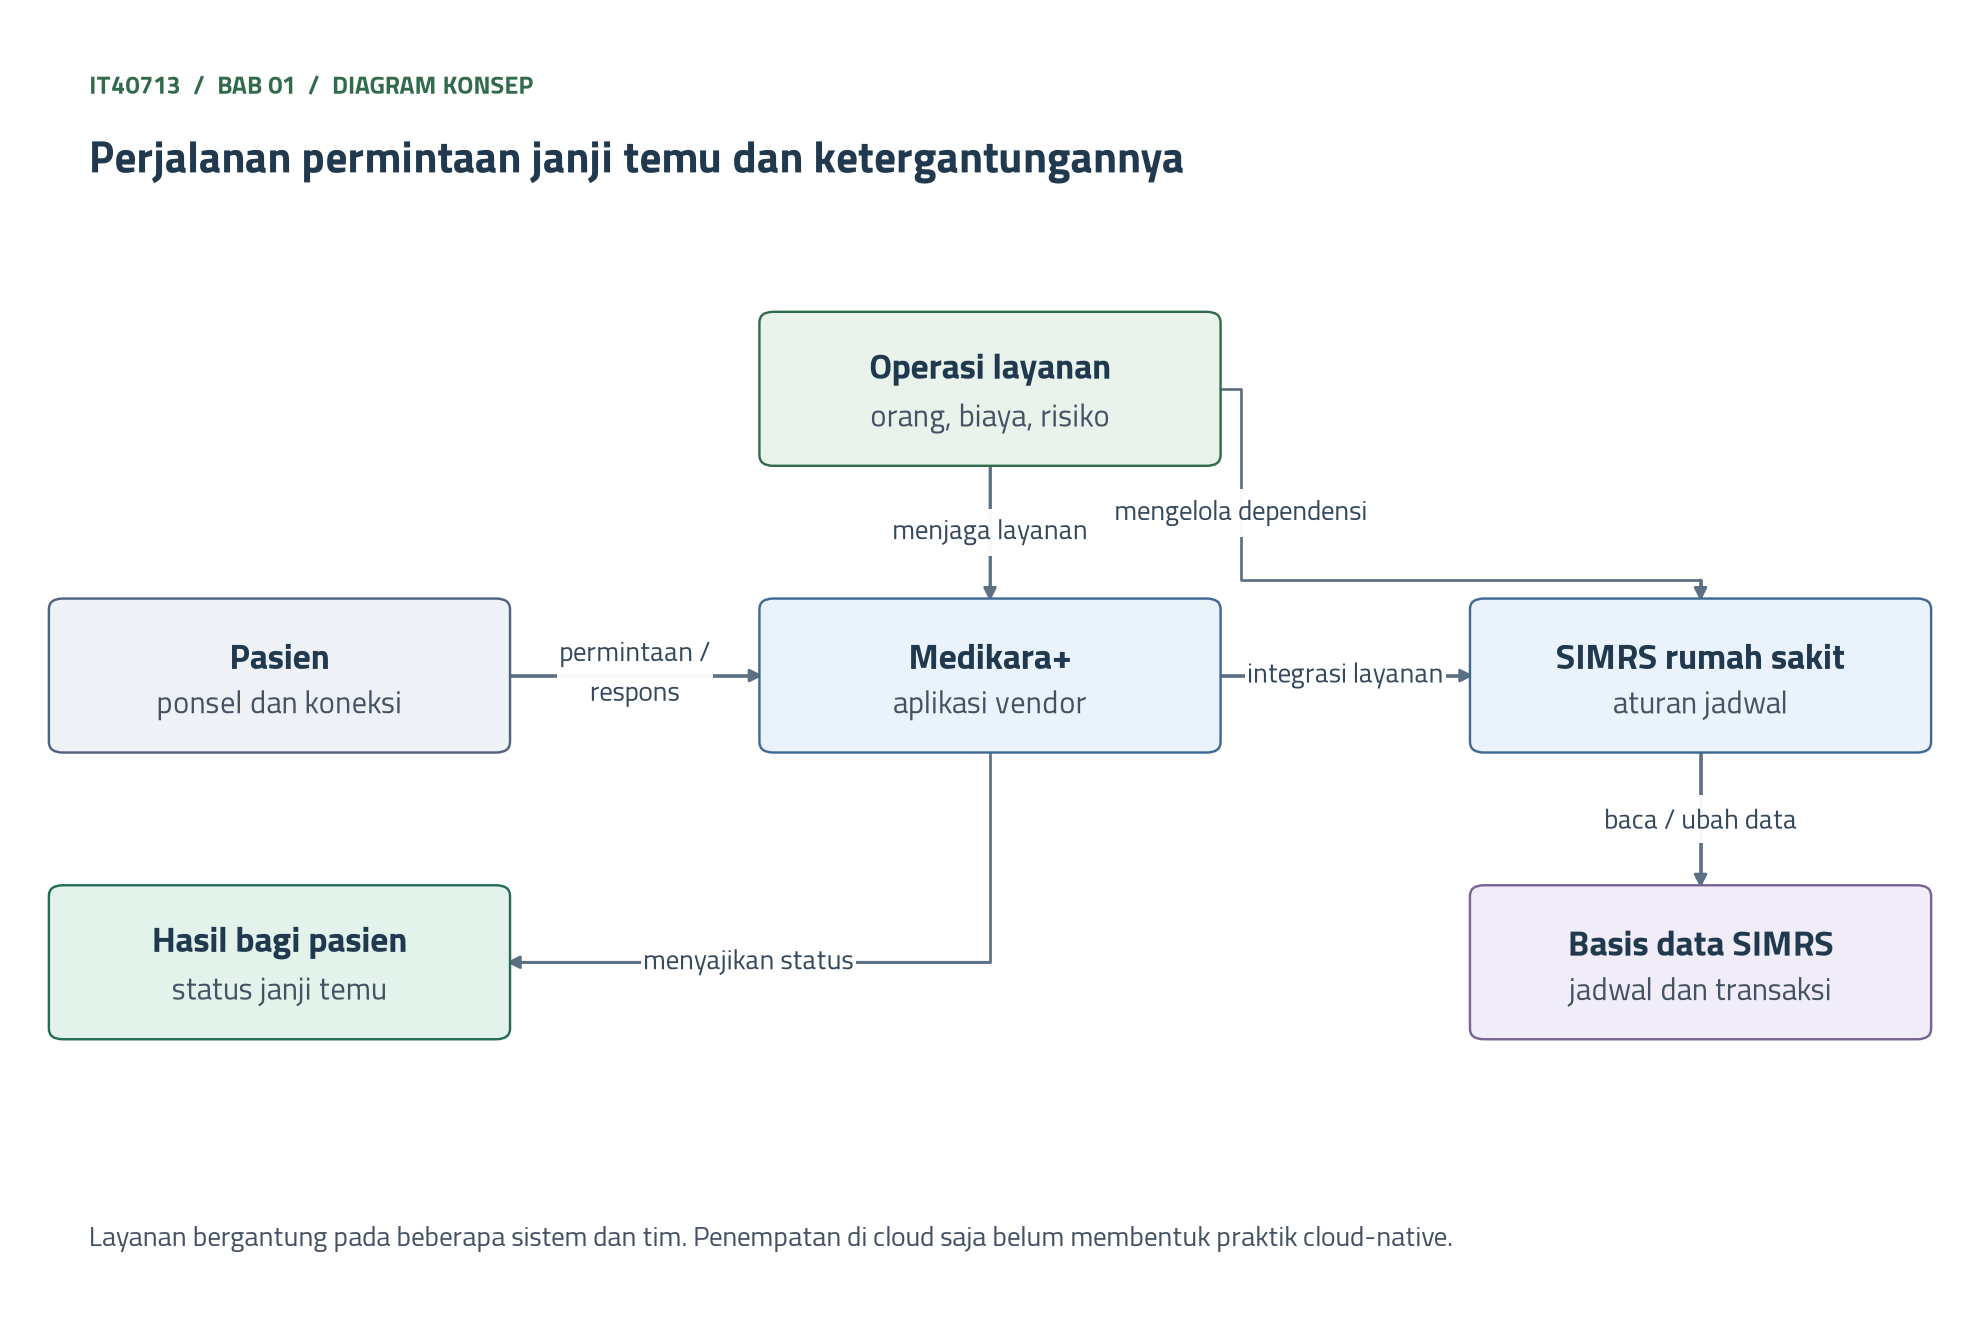
\includegraphics[width=0.96\textwidth,height=0.77\textheight,keepaspectratio]{../../figures/ch01-diagram-konsep.png}
\end{frame}

\begin{frame}{Enam Istilah Dasar}
  \footnotesize
  \begin{tabularx}{\textwidth}{>{\raggedright\arraybackslash}p{2cm}
                               >{\raggedright\arraybackslash}X
                               >{\raggedright\arraybackslash}p{3.3cm}}
    \hline
    \textbf{Istilah} & \textbf{Arti sederhana} & \textbf{Analogi} \\
    \hline
    Aplikasi & Program untuk menyelesaikan pekerjaan & Ruang makan dan menu \\
    \hline
    Server & Komputer yang menjalankan aplikasi bagi banyak pengguna & Dapur dan koki \\
    \hline
    Basis data & Tempat data disimpan teratur & Gudang bahan dan buku stok \\
    \hline
    Jaringan & Jalur yang menghubungkan perangkat & Jalan raya \\
    \hline
    Pusat data & Ruang server dengan listrik cadangan dan pendingin & Gudang
      berpendingin dengan genset \\
    \hline
    \textit{Cloud} & Layanan komputasi yang disewa sesuai pemakaian & Menyewa mobil \\
    \hline
  \end{tabularx}
\end{frame}

\begin{frame}{Cloud sebagai Layanan Komputasi yang Disewa}
  \begin{itemize}
    \item NIST: akses lewat jaringan ke kumpulan sumber daya komputasi bersama,
          disediakan dan dilepas dengan cepat.
    \item Lima karakteristik: swalayan, akses jaringan luas, penggabungan sumber
          daya, elastisitas cepat, layanan terukur.
    \item Analogi: menyewa mobil. Bayar sesuai pakai, tetapi pemakaian harian jarak
          jauh bisa lebih murah dengan membeli.
    \item Contoh: puncak Medikara+ Senin pagi 4 kali rata-rata; kapasitas tambahan
          disewa hanya saat puncak.
    \item Tanggung jawab atas data dan cara pemakaian tidak ikut berpindah.
  \end{itemize}
\end{frame}

\begin{frame}{Perjalanan Satu Permintaan Janji Temu}
  \centering
  \resizebox{0.88\textwidth}{!}{% Perjalanan satu permintaan janji temu dari aplikasi Medikara+ sampai ke basis
% data SIMRS rumah sakit, lalu jawabannya kembali ke ponsel pasien.
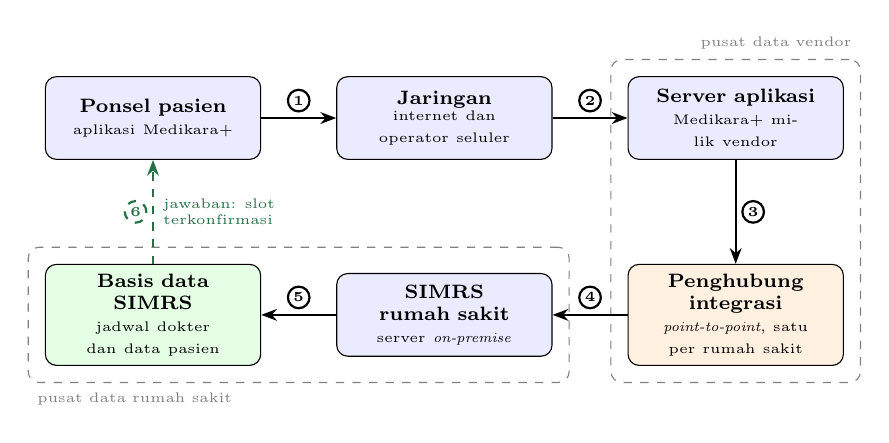
\begin{tikzpicture}[
  font=\scriptsize,
  kotak/.style={draw, rounded corners, align=center, minimum height=1.05cm,
                text width=2.5cm},
  nomor/.style={circle, draw, fill=white, inner sep=1pt, font=\tiny\bfseries},
  panah/.style={-{Stealth[length=2mm]}, thick}
]
  \node[kotak, fill=blue!8] (ponsel) at (0,0)
    {\textbf{Ponsel pasien}\\{\tiny\mdseries aplikasi Medikara+}};
  \node[kotak, fill=blue!8] (jaringan) at (3.7,0)
    {\textbf{Jaringan}\\{\tiny\mdseries internet dan\\operator seluler}};
  \node[kotak, fill=blue!8] (aplikasi) at (7.4,0)
    {\textbf{Server aplikasi}\\{\tiny\mdseries Medikara+ milik vendor}};
  \node[kotak, fill=orange!12] (integrasi) at (7.4,-2.5)
    {\textbf{Penghubung integrasi}\\{\tiny\mdseries \textit{point-to-point}, satu per rumah sakit}};
  \node[kotak, fill=blue!8] (simrs) at (3.7,-2.5)
    {\textbf{SIMRS rumah sakit}\\{\tiny\mdseries server \textit{on-premise}}};
  \node[kotak, fill=green!10] (basisdata) at (0,-2.5)
    {\textbf{Basis data SIMRS}\\{\tiny\mdseries jadwal dokter dan data pasien}};

  \begin{scope}[on background layer]
    \node[draw, dashed, gray, rounded corners, inner sep=6pt,
          fit=(aplikasi) (integrasi)] (vendor) {};
    \node[draw, dashed, gray, rounded corners, inner sep=6pt,
          fit=(simrs) (basisdata)] (rumahsakit) {};
  \end{scope}
  \node[font=\tiny, gray, anchor=south east] at (vendor.north east) {pusat data vendor};
  \node[font=\tiny, gray, anchor=north west] at (rumahsakit.south west)
    {pusat data rumah sakit};

  \draw[panah] (ponsel) -- node[nomor, above=2pt] {1} (jaringan);
  \draw[panah] (jaringan) -- node[nomor, above=2pt] {2} (aplikasi);
  \draw[panah] (aplikasi) -- node[nomor, right=2pt] {3} (integrasi);
  \draw[panah] (integrasi) -- node[nomor, above=2pt] {4} (simrs);
  \draw[panah] (simrs) -- node[nomor, above=2pt] {5} (basisdata);
  \draw[panah, dashed, praditagreen] (basisdata.north) -- node[nomor, left=2pt] {6}
    node[pos=0.5, right, font=\tiny, text=praditagreen, align=left]
      {jawaban: slot\\terkonfirmasi} (ponsel.south);
\end{tikzpicture}
}
\end{frame}

\begin{frame}{Kasus Medikara Health: Keluhan adalah Gejala}
  \begin{itemize}
    \item Pasien menunggu 25 detik lalu gagal memesan. Yang terasa: "aplikasinya
          lambat".
    \item Penyebabnya bisa di enam titik: sinyal, jaringan, server vendor,
          penghubung, SIMRS, atau basis data.
    \item Lima versi SIMRS berarti lima penghubung berbeda.
    \item Perubahan di satu SIMRS berpotensi merusak satu penghubung.
    \item Daftar pemicu modernisasi memisahkan keluhan dari dugaan penyebab.
  \end{itemize}
\end{frame}

\section{Bahasa Bersama Teknis}

\begin{frame}{\hfill}
  \centering
  \Huge{\textbf{Bahasa Bersama untuk\\Mahasiswa Teknis}}
\end{frame}

\begin{frame}{Nilai Bisnis dan Cara Manajemen Menilainya}
  \begin{itemize}
    \item Nilai bisnis: pendapatan naik, biaya turun, risiko mengecil, pelanggan
          puas, kepatuhan terjaga.
    \item Diukur lewat KPI: waktu tunggu, jumlah kunjungan, biaya per kunjungan.
    \item Analogi: pemilik warung kopi bertanya cangkir tambahan dan masa balik
          modal, bukan tekanan uap.
    \item "Memperbarui server SIMRS Bekasi" menjadi "memangkas waktu tunggu dari 70
          menjadi 30 menit".
    \item Telekonsultasi: 60 sesi × Rp150.000 = Rp9 juta hilang per jam henti pada
          jam sibuk.
  \end{itemize}
\end{frame}

\begin{frame}{Dari Bahasa Teknis ke Bahasa Dampak}
  \footnotesize
  \begin{tabularx}{\textwidth}{>{\raggedright\arraybackslash}X
                               >{\raggedright\arraybackslash}p{3.2cm}
                               >{\raggedright\arraybackslash}X}
    \hline
    \textbf{Bahasa teknis} & \textbf{Pertanyaan direksi} & \textbf{Bahasa dampak} \\
    \hline
    Server SIMRS Bekasi sering kehabisan memori & Apa akibatnya bagi pasien? &
      Pendaftaran berhenti 3 kali sebulan, masing-masing sekitar 40 menit \\
    \hline
    Integrasi \textit{point-to-point} ke lima SIMRS & Berapa biayanya? & Satu kerja
      sama baru tertunda sekitar 4 bulan \\
    \hline
    Akun vendor tanpa masa berlaku & Seberapa besar risikonya? & Jalur insiden 2025;
      wajib lapor dalam 3 kali 24 jam \\
    \hline
    Laporan dari \textit{spreadsheet} & Apa yang hilang? & Laporan baru siap tanggal
      12, keputusan terlambat dua pekan \\
    \hline
  \end{tabularx}
\end{frame}

\begin{frame}{Struktur Biaya: CapEx dan OpEx}
  \begin{itemize}
    \item CapEx: aset dibayar di muka dan disusutkan; OpEx: dibayar selama layanan
          dipakai.
    \item Pindah ke \textit{cloud} menggeser sebagian biaya dari CapEx ke OpEx.
    \item Analogi: membeli mesin fotokopi Rp60 juta atau menyewa dengan tarif per
          lembar.
    \item 6 server SIMRS Bandung Rp1,8 miliar (Rp360 juta per tahun selama 5 tahun)
          dibandingkan \textit{cloud} Rp32 juta per bulan: keputusan menunggu TCO.
    \item Tagihan Medikara+ naik 46 persen (Rp28 juta menjadi Rp41 juta): perlu label
          biaya per layanan.
  \end{itemize}
\end{frame}

\begin{frame}{Risiko dan Kepatuhan sebagai Batasan Desain}
  \begin{itemize}
    \item UU PDP: data kesehatan termasuk data pribadi spesifik.
    \item Kegagalan pelindungan wajib diberitahukan paling lambat 3 kali 24 jam;
          denda administratif paling tinggi 2 persen pendapatan tahunan.
    \item Permenkes 24/2022: rekam medis elektronik wajib sejak 31 Desember 2023;
          boleh disimpan di \textit{cloud} tersertifikasi.
    \item Analogi: tangga darurat ditentukan saat denah digambar, bukan setelah
          gedung berdiri.
  \end{itemize}
\end{frame}

\begin{frame}{Kasus Medikara Health: Insiden Vendor dan Audit}
  \begin{itemize}
    \item 2025: data sebagian pasien Medikara+ terbuka lewat akun uji vendor yang
          masih aktif.
    \item Audit internal: akun mantan karyawan masih aktif, akun dipakai bersama.
    \item Batasan 1: setiap akun punya hak minimum dan masa berlaku.
    \item Batasan 2: setiap akses ke data pasien tercatat dan dapat diaudit.
    \item Batasan 3: data terdampak diketahui kurang dari 3 kali 24 jam, sehingga
          butuh katalog data.
  \end{itemize}
\end{frame}

\begin{frame}{Menulis Rekomendasi untuk Direksi}
  \begin{itemize}
    \item Satu halaman, jawaban di depan (prinsip piramida), berbasis dampak.
    \item Menyebut pilihan lain, \textit{trade-off}, dan keputusan yang diminta.
    \item Lemah: "migrasi SIMRS ke \textit{microservices} di Kubernetes agar
          \textit{scalable}".
    \item Kuat: "setujui uji coba pendaftaran daring terpadu di Bekasi, 3 bulan,
          Rp420 juta, sasaran 70 menjadi 30 menit".
    \item Analogi: dokter menjelaskan pilihan tindakan kepada keluarga pasien.
  \end{itemize}
\end{frame}

\section{Kualitas Sistem dan Trade-off}

\begin{frame}{\hfill}
  \centering
  \Huge{\textbf{Kualitas Sistem dan\\Trade-off}}
\end{frame}

\begin{frame}{Lima Kualitas Sistem}
  \footnotesize
  \begin{tabularx}{\textwidth}{>{\raggedright\arraybackslash}p{3cm}
                               >{\raggedright\arraybackslash}X
                               >{\raggedright\arraybackslash}X}
    \hline
    \textbf{Kualitas} & \textbf{Pertanyaan} & \textbf{Contoh di Medikara Health} \\
    \hline
    Ketersediaan & Bisakah dipakai saat dibutuhkan? & SIMRS instalasi gawat darurat
      24 jam \\
    \hline
    Skalabilitas & Sanggupkah melayani beban yang bertambah? & Lonjakan janji temu
      Senin pagi \\
    \hline
    Keamanan & Terlindungkah data dan akses? & Akun vendor dan mantan karyawan \\
    \hline
    Biaya & Berapa yang dibayar untuk hasil itu? & Tagihan \textit{cloud} Medikara+ \\
    \hline
    Kecepatan perubahan & Seberapa cepat perubahan sampai ke pengguna? & Fitur
      menunggu jadwal rilis vendor \\
    \hline
  \end{tabularx}
\end{frame}

\begin{frame}{Kualitas Saling Tarik-Menarik}
  \centering
  \resizebox{!}{0.68\textheight}{% Lima kualitas sistem yang saling tarik-menarik. Setiap sisi segi lima
% menandai satu pasangan yang sering bertentangan, dengan contoh singkatnya.
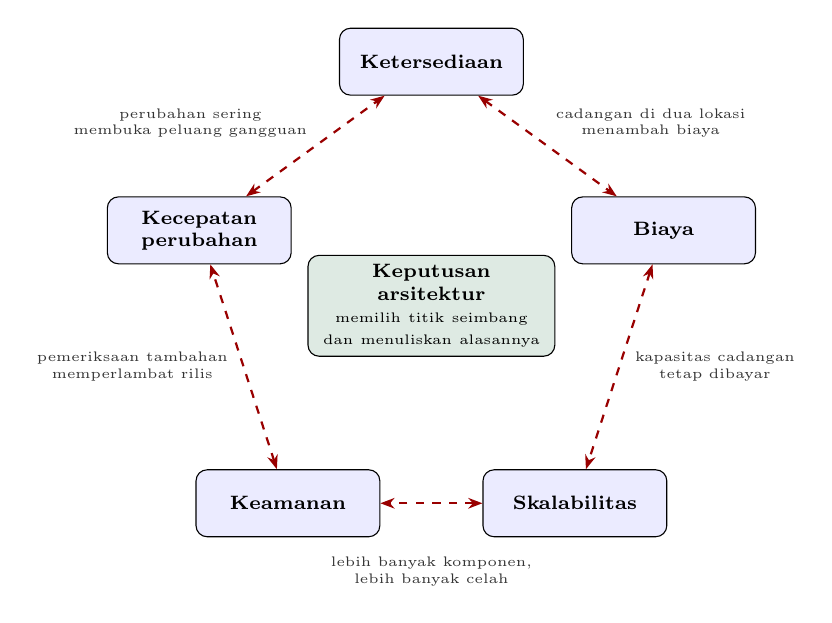
\begin{tikzpicture}[
  font=\scriptsize,
  kualitas/.style={draw, rounded corners, align=center, minimum height=0.85cm,
                   text width=2.1cm, fill=blue!8, font=\scriptsize\bfseries},
  tarik/.style={{Stealth[length=1.8mm]}-{Stealth[length=1.8mm]}, thick, red!60!black,
                dashed},
  catatan/.style={font=\tiny, gray!40!black, align=center}
]
  \node[kualitas] (sedia) at (90:3.1) {Ketersediaan};
  \node[kualitas] (biaya) at (18:3.1) {Biaya};
  \node[kualitas] (skala) at (-54:3.1) {Skalabilitas};
  \node[kualitas] (aman) at (-126:3.1) {Keamanan};
  \node[kualitas] (ubah) at (162:3.1) {Kecepatan\\perubahan};

  \node[draw, rounded corners, align=center, fill=praditagreen!15, text width=2.9cm,
        minimum height=1.1cm, font=\scriptsize] at (0,0)
    {\textbf{Keputusan arsitektur}\\[2pt]
     {\tiny\mdseries memilih titik seimbang\\dan menuliskan alasannya}};

  \draw[tarik] (sedia) -- node[catatan, above right=-1pt] {cadangan di dua lokasi\\menambah biaya} (biaya);
  \draw[tarik] (biaya) -- node[catatan, right=2pt] {kapasitas cadangan\\tetap dibayar} (skala);
  \draw[tarik] (skala) -- node[catatan, below=0.55cm] {lebih banyak komponen,\\lebih banyak celah} (aman);
  \draw[tarik] (aman) -- node[catatan, left=2pt] {pemeriksaan tambahan\\memperlambat rilis} (ubah);
  \draw[tarik] (ubah) -- node[catatan, above left=-1pt] {perubahan sering\\membuka peluang gangguan} (sedia);
\end{tikzpicture}
}
\end{frame}

\begin{frame}{Target Ketersediaan dan Waktu Henti}
  \small
  \begin{tabularx}{\textwidth}{>{\raggedright\arraybackslash}p{2.6cm}
                               >{\raggedright\arraybackslash}X
                               >{\raggedright\arraybackslash}X}
    \hline
    \textbf{Target} & \textbf{Henti per tahun} & \textbf{Henti per bulan (30 hari)} \\
    \hline
    99\% & 87,6 jam (sekitar 3,65 hari) & 7,2 jam \\
    \hline
    99,5\% & 43,8 jam & 3,6 jam \\
    \hline
    99,9\% & 8,76 jam & 43,2 menit \\
    \hline
    99,95\% & 4,38 jam & 21,6 menit \\
    \hline
    99,99\% & 52,6 menit & 4,3 menit \\
    \hline
  \end{tabularx}

  \vspace{8pt}
  Setiap angka sembilan tambahan memangkas waktu henti, tetapi biayanya naik lebih
  cepat daripada manfaatnya.
\end{frame}

\begin{frame}{Menuliskan Alasan Keputusan}
  \begin{itemize}
    \item \textbf{Konteks:} telekonsultasi kehilangan sekitar Rp9 juta per jam henti.
    \item \textbf{Keputusan:} target 99,9 persen, dua lokasi dalam satu region.
    \item \textbf{Alasan:} 99,99 persen menuntut dua region; biayanya melebihi
          kerugian yang dicegah.
    \item \textbf{\textit{Trade-off}:} bila seluruh region terganggu, layanan dapat
          berhenti beberapa jam.
    \item \textbf{Tanggal dan pemutus:} Januari 2026, direktur operasional dan kepala
          divisi TI.
  \end{itemize}
\end{frame}

\section{Arti Cloud-Native bagi Organisasi}

\begin{frame}{\hfill}
  \centering
  \Huge{\textbf{Arti Cloud-Native\\bagi Organisasi}}
\end{frame}

\begin{frame}{Cloud-Hosted dan Cloud-Native}
  \footnotesize
  \begin{tabularx}{\textwidth}{>{\raggedright\arraybackslash}p{3cm}
                               >{\raggedright\arraybackslash}X
                               >{\raggedright\arraybackslash}X}
    \hline
    \textbf{Aspek} & \textbf{\textit{Cloud-hosted}} & \textbf{\textit{Cloud-native}} \\
    \hline
    Bentuk aplikasi & Sama seperti di pusat data lama & Dirancang ulang, longgar
      keterkaitannya \\
    \hline
    Menambah kapasitas & Manual & Otomatis mengikuti beban \\
    \hline
    Cara rilis & Jarang dan berisiko besar & Sering, kecil, otomatis \\
    \hline
    Saat gangguan & Satu kesalahan menghentikan semua & Dibatasi pada satu bagian \\
    \hline
    Yang berubah & Lokasi server & Lokasi, rancangan, dan cara kerja tim \\
    \hline
  \end{tabularx}

  \vspace{8pt}
  \small Analogi: warung yang pindah ke mal tanpa mengubah cara kerja tetap punya
  satu kasir dan antrean panjang.
\end{frame}

\begin{frame}{Lima Mitos dan Kenyataannya}
  \footnotesize
  \begin{tabularx}{\textwidth}{>{\raggedright\arraybackslash}p{4.2cm}
                               >{\raggedright\arraybackslash}X}
    \hline
    \textbf{Mitos} & \textbf{Kenyataan} \\
    \hline
    \textit{Cloud} selalu lebih murah & Survei Flexera 2026: sekitar 29 persen belanja
      \textit{cloud} diperkirakan terbuang \\
    \hline
    \textit{Microservices} selalu lebih baik & Segment menggabungkan kembali ratusan
      layanan kecilnya menjadi satu \\
    \hline
    Pindah ke \textit{cloud} otomatis aman & Akun, hak akses, dan konfigurasi tetap
      tanggung jawab pelanggan \\
    \hline
    \textit{Cloud-native} berarti Kubernetes & Definisi CNCF menekankan praktik, bukan
      alat \\
    \hline
    Sekali pindah, urusan selesai & Modernisasi bertahap, dikelola sebagai peta jalan \\
    \hline
  \end{tabularx}
\end{frame}

\begin{frame}{Perjalanan Mata Kuliah}
  \centering
  \resizebox{0.95\textwidth}{!}{% Perjalanan mata kuliah IT40713 dalam empat Bagian, dari strategi sampai peta
% jalan, beserta pertanyaan utama yang dijawab tiap Bagian.
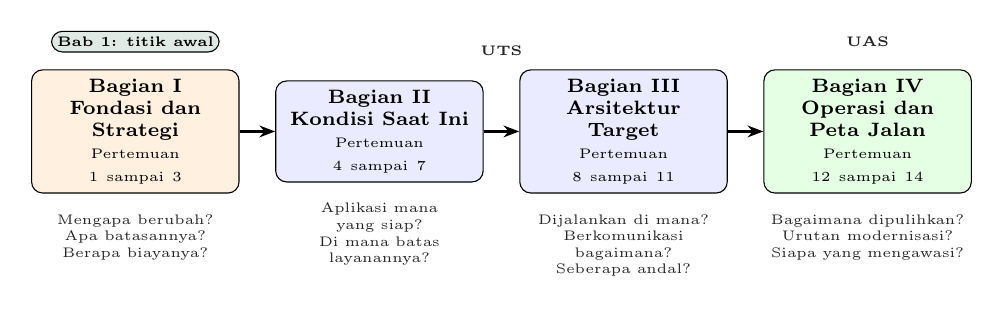
\begin{tikzpicture}[
  font=\scriptsize,
  bagian/.style={draw, rounded corners, align=center, minimum height=1.15cm,
                 text width=2.4cm, font=\scriptsize\bfseries},
  tanya/.style={align=center, text width=2.5cm, font=\tiny, gray!30!black},
  panah/.style={-{Stealth[length=2mm]}, thick}
]
  \node[bagian, fill=orange!12] (b1) at (0,0)
    {Bagian I\\Fondasi dan Strategi\\{\tiny\mdseries Pertemuan 1 sampai 3}};
  \node[bagian, fill=blue!8] (b2) at (3.1,0)
    {Bagian II\\Kondisi Saat Ini\\{\tiny\mdseries Pertemuan 4 sampai 7}};
  \node[bagian, fill=blue!8] (b3) at (6.2,0)
    {Bagian III\\Arsitektur Target\\{\tiny\mdseries Pertemuan 8 sampai 11}};
  \node[bagian, fill=green!10] (b4) at (9.3,0)
    {Bagian IV\\Operasi dan Peta Jalan\\{\tiny\mdseries Pertemuan 12 sampai 14}};

  \draw[panah] (b1) -- (b2);
  \draw[panah] (b2) -- (b3);
  \draw[panah] (b3) -- (b4);

  \node[tanya, below=4pt of b1] {Mengapa berubah?\\Apa batasannya?\\Berapa biayanya?};
  \node[tanya, below=4pt of b2] {Aplikasi mana yang siap?\\Di mana batas\\layanannya?};
  \node[tanya, below=4pt of b3] {Dijalankan di mana?\\Berkomunikasi bagaimana?\\Seberapa andal?};
  \node[tanya, below=4pt of b4] {Bagaimana dipulihkan?\\Urutan modernisasi?\\Siapa yang mengawasi?};

  \node[draw, fill=praditagreen!15, rounded corners, font=\tiny\bfseries,
        inner sep=2pt] (bab1) at ([yshift=10pt]b1.north) {Bab 1: titik awal};
  \node[font=\tiny\bfseries, gray!30!black] at ($(b2.north)!0.5!(b3.north)+(0,0.3)$) {UTS};
  \node[font=\tiny\bfseries, gray!30!black] at ([yshift=10pt]b4.north) {UAS};
\end{tikzpicture}
}
\end{frame}

\begin{frame}{Kasus Medikara Health: Satu Pasien, Satu Rekam Medis}
  \begin{itemize}
    \item Di mana rekam medis terpadu disimpan, dan aturan apa yang membatasinya?
          (Bab 2)
    \item Berapa biaya infrastruktur per kunjungan pasien? (Bab 3)
    \item Lima SIMRS diseragamkan, diganti, atau dibungkus? (Bab 4 sampai 7)
    \item Bagaimana mitra tersambung tanpa \textit{point-to-point} baru? (Bab 9)
    \item Bagaimana rekam medis dipulihkan bila satu pusat data padam? (Bab 12)
  \end{itemize}
\end{frame}

\section{Aktivitas}

\begin{frame}{Aktivitas: Membentuk Tim dan Memetakan Pemicu}
  \begin{itemize}
    \item Tim 3 sampai 5 orang, sedikitnya satu anggota teknis dan satu non-teknis.
    \item Peran: koordinator, pemimpin wawancara (non-teknis), pemeta sistem
          (teknis), serta penjaga izin dan etika.
    \item Pemicu modernisasi: masalah nyata, lengkap dengan dampak berangka dan
          sistem yang terlibat.
    \item Penilaian: kejelasan masalah 30\%, keterkaitan sistem 25\%, dampak terukur
          25\%, etika 20\%.
  \end{itemize}
\end{frame}

\begin{frame}{Langkah Kerja dan Luaran}
  \small
  \begin{enumerate}
    \item Bentuk tim dan tetapkan peran.
    \item Pilih organisasi dan urus izin, atau pakai Medikara Health.
    \item Wawancarai 3 sampai 5 narasumber, sekitar 20 menit per orang.
    \item Petakan sistem yang terlibat dalam setiap masalah.
    \item Tulis profil satu halaman dan 5 sampai 10 pemicu modernisasi (C1).
  \end{enumerate}
  \vspace{4pt}
  {\footnotesize Berkas: \berkas{sources/chapter01/templat-profil-organisasi.md},
  \berkas{sources/chapter01/lembar-pemicu-modernisasi.md},
  \berkas{sources/chapter01/panduan-izin-dan-anonimisasi.md}}
\end{frame}

\section{Ringkasan dan Latihan}

\begin{frame}{Ringkasan}
  \begin{itemize}
    \item Pindah ke \textit{cloud} tidak otomatis menyelesaikan masalah; penyebabnya
          perlu dipisahkan lebih dahulu.
    \item Empat mata kuliah menyusun satu cetak biru lewat tonggak C1 sampai C4.
    \item Bahasa bersama: istilah dasar sistem bagi non-teknis, nilai bisnis dan
          risiko bagi teknis.
    \item Kualitas sistem saling tarik-menarik; alasan setiap keputusan ditulis.
    \item \textit{Cloud} adalah alat, bukan tujuan.
  \end{itemize}
\end{frame}

\begin{frame}{Latihan}
  \begin{enumerate}
    \item \textbf{\textit{Cloud-hosted} dan \textit{cloud-native}:} bandingkan
          satu aplikasi pada lima aspek dalam dua skenario.
    \item \textbf{Dua sisi satu masalah:} antrean Bekasi, sekitar 18 pasien pulang
          tiap Senin, sekitar Rp327,6 juta per tahun.
    \item \textbf{Biaya dan ketersediaan:} pilihan 99,5\%, 99,9\%, dan 99,99\% untuk
          telekonsultasi. Total terendah: 99,9\%, sekitar Rp654,8 juta per tahun.
  \end{enumerate}
  \vspace{4pt}
  {\small Tabel contoh dan lembar isian ada di Bab 1 modul.}
\end{frame}

\end{document}
